\chapter{Background} \label{ch:background}

This chapter provides an extensive discussion on network control in
packet-switched networks.  We motivate the discussion on network control,
describing the architecture of network devices and their inherent physical
limitations (Section~\ref{sec:background:forwarding}) and elaborate on existing
network control mechanisms for production networks
(Section~\ref{sec:background:netcontrol}).  Furthermore, we present three
significant efforts in flexible network control, namely Active Networks,
Devolved Control of ATM Networks (DCAN) and Software Defined Networking (SDN),
proposed by the research community to address limitations in network control
schemes (Section~\ref{sec:background:netcontrol}). Finally, we focus on the SDN
paradigm and present some of its applications in a series of current network
problems (Section~\ref{sec:background:ofapp}).

\section{Forwarding Devices} \label{sec:background:forwarding}

In this section we focus on Ethernet networks and provide a high-level design
overview of a common forwarding device, a \emph{switch}. Using this model we
highlight the physical limits of network control and motivate a discussion on
effective control. 

% Providing a high level
% insight on the architecture of a Switch, can highlight the existing lower bounds
% on the functionality and extendibility of such devices. 

\begin{figure}
  \centering
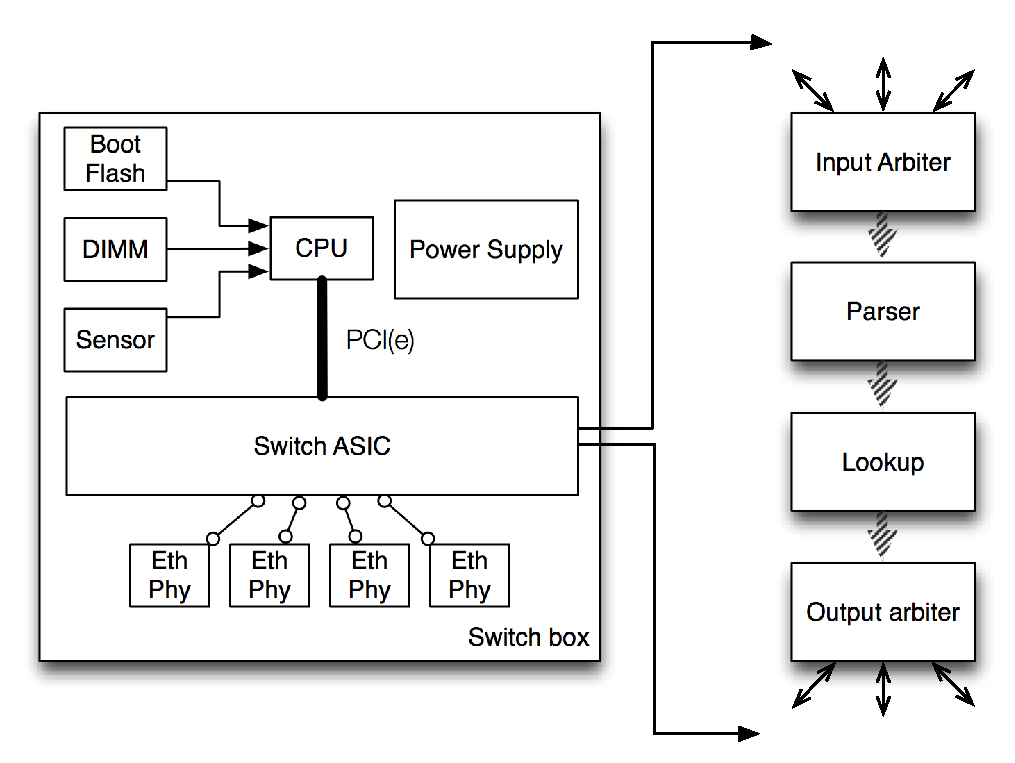
\includegraphics[width=0.6\textwidth]{Background/BackgroundFigs/switch_design}
\caption{A generic switch design model.}
\label{fig:background:switch_design}
\end{figure}

Ethernet switches multiplex Ethernet broadcast domains and provide
collision-free connectivity between network segments.  Network vendors provide
a wide range of switch type with variable functional capabilities (e.g. VLAN
support, multilayer switches).  For example, an unmanaged switch provides
elementary non-configurable functionality with low 1 GbE port density, while a
distribution switch provides high 10 or 40 GbE port density and a range of
traffic management applications.  We use the Top-of-Rack~(ToR) switch type to
elaborate on the architecture of modern hardware switches.  ToR switches are
used in datacenter and enterprise networks to multiplex traffic between the
edge and the distribution network layers. Forwarding functionality is
implemented  using an Application-Specific Integrated Circuit~(ASIC) silicon,
providing multi-GbE line-rate non-blocking traffic forwarding.
Figure~\ref{fig:background:switch_design} presents the ToR architecture
which consists of the following components:

\begin{itemize}
  \item \emph{co-processor/management CPU}: Switch devices use a programmable
    CPU to fulfil control plane computation requirements. The CPU hosts a
    minimal operating system, responsible to translate the device configuration in
    appropriate ASIC manipulation at run-time. Vendors usually employ low-power CPUs, like SoC
    PowerPC and ARM processors. The CPU is equipped with runtime
    (Boot Flash and RAM) and persistent (e.g.~SD Cards) memory modules. In general,
    switch CPUs provide sufficient computation resources to run the switch
    control-plane functionality, but they cannot accommodate intensive processing
    tasks. The OS provides elementary remote control services, like telnet and SSH,
    command line/web interfaces and SNMP access to the switch state. 
 
  \item \emph{Switch ASIC}: The switch ASIC~\mycite{hp-asic,broadcom-asic,intel-asic}
    implements in hardware the data plane functionality  The capabilities of
    an ASIC are variable, depending on the vendor and the cost, and define the data
    plane performance limits of the device.  ASICs have an expensive
    development cycle, consisting of long design and
    testing periods, and require significant human labour and material resource
    requirements. As a result, innovation has a high latency to
    reach the production and the design details remain undisclosed.  

    The ASIC packet processing pipeline commonly contains four modules.  The
    \emph{input arbiter} module multiplexes and synchronizes packets from the
    Ethernet ports to the main processing pipeline of the silicon. The arbiter
    ensures non pre-emptive packet processing, by bridging the mismatch
    between the silicon processing clock rate and the link rate. The pipeline 
    contains also a \emph{protocol parsing} module and an
    \emph{memory lookup} module. The protocol parser extracts significant packet
    fields from network packets, used by the memory lookup module
    to define packet processing and forwarding.  The lookup module
    uses a memory module, integrated or external to ASIC, which contains 
    the forwarding policy.  Memory modules have a trade-off
    between cost and access speed and between memory cost and memory management
    complexity~\footnote{CAM/TCAM lookup: $<$ 10 clock cycles, SRAM: 2-3 nsec,
      DRAM: 20-35
      nsec,~\url{http://people.ee.duke.edu/~sorin/prior-courses/ece152-spring2009/lectures/6.2.2-memory.pdf}}.
    Finally, the \emph{output arbiter} module is responsible to apply modifications
    to the packet and forward it to the appropriate output queue.
    The processing pipeline may contain additional modules
    which extend the functionality providing
    access control list (ACL) virtual network queues and flow statistics
    monitoring.

  \item \emph{ASIC-CPU interconnection}: The management CPU is connected with the ASIC
    over a PCI or PCI-express channel. The interconnection provides an
    elementary bi-directional channel allowing the CPU to program the ASIC
    through its register API and the ASIC to propagate exceptional packets to
    the CPU\@. The channel provides sufficient bandwidth for basic control plane
    communication, but it is not designed to handle high rate information. For
    example, current broadcom trident chipsets use a PCIe 4x or 8x bus,
    achieving 2 to 4 Gbps capacity.  

  \item \emph{Memory}: Apart from in-ASIC memory modules, switches
    also use multiple memory types to support the run-time requirements of the
    firmware. A switch is usually equipped with CPU Boot Flash, to boot the
    OS/firmware, DIMM RAM and multiple memory slots, for control plane logging
    and configuration persistence.

  \item \emph{Ethernet ports} : The receipt and transmission of Ethernet packets
    is implemented by a separate hardware module, 
    implementing the physical and MAC layers of the protocol. The port module 
    connects with the  ASIC through a Media Independent Interface (MII) and
    contains small packet buffers to reduce packet loss.  
\end{itemize}

In terms of data plane performance,  the forwarding capabilities of an ASIC are
upper-bound by the transistor density and size, as in general purpose CPU
silicones. A ToR switch uses a single ASIC, supporting up to 100 Gbps processing
capacity.  In terms of control plane performance, the primary limitation is the
capacity of the communication bus between the coprocessor and the ASIC, the
design of the interface between the two entities and the processing capabilities
of the switch CPU\@.  For a ToR switch, the vendors usually provide a PCIe
communication bus, supporting capacities on the order of a few Gigabytes, while
CPUs are usually constrained (Section~\ref{sec:oflops:switches} provide details
on some of-the-self ToR switches).

ToR switches are simple switch devices and provide low to medium forwarding
capacity. Vendors provide network devices supporting higher link capacities and
enhanced functionalities, which have more complex architectures. Multi-chassis
switches and routers, used in the core of large networks, cannot fit their
processing pipeline requirements in a single ASIC\@.  Packet processing is
distributed between multiple silicons, interconnected using complex CLOS
crossbar fabrics with non-blocking Terabit backplane
capacities~\mycite{juniper_t_series}. Network control in such devices exhibits
similar high complexity and uses distributed forwarding tables and cache
coherent protocols to ensure state consistency~\mycite{cisco_cef}. In such
devices, ASIC control is complex, inflexible and slow.  

\section{Forwarding Control in Production Networks} \label{sec:background:netcontrol}

Current network architectures and technologies set dynamic control as a
fundamental design goal.  Existing standardized approaches provide
\textit{distributed}, \textit{autonomous} and \textit{resilient} control,
influenced extensively by the end-to-end Internet principle. The administrator
is responsible to define the local policy of a device and at run-time
distributed protocols reconstruct the global network state.  Using the global
network state, the forwarding logic determines an optimal forwarding policy
which optimizes specific aspects of network performance.  For the rest of this
section we present the control plane functionality in the data link and network
layers of the network stack. 
% existing production-level protocols that enable distributed network control. We
% focus on the Data-Link and Network layer protocols as these layer define the
% hop-by-hop forwarding policy.

\subsection{Data-Link Layer Control}

Data-Link layer control protocols provide loop-detection, VLAN and QoS
configuration automation. Loop detection is used to avoid packet loops in
networks with redundant connectivity, since the Ethernet specification doesn't
support packet timeout functionality.  The Spanning Tree Protocol~(STP) was a
first attempt to address this problem, standardised by IEEE in
802.1D-1998~\mycite{ieee_802_1d_1998}. The protocol implements the distributed
spanning tree construction algorithm, presented in~\mycite{Perlman1985}. The
algorithm uses broadcast messages to discover a spanning tree over the network
graph, with respect to a common root switch. For each port, the switch maintains
a state machine, which disables packet forwarding when the respective link is
not part of the spanning tree.  Because the initial definition of the protocol
faced significant convergence delay after a network change, IEEE introduce the
Rapid Spanning Tree Protocol~(RSTP), an evolved version of
STP~\mycite{ieee_802_1d_2004}.  In addition,  IEEE Multiple Spanning Tree
Protocol~(MSTP)~\mycite{ieee_802_1q} develops a modified version of the protocol,
optimized for VLAN-based networks. MSTP constructs a spanning trees for each
VLAN, which effectively  reduce unnecessary port blocking. Cisco has developed a
series of proprietary protocols to address the problem in a similar
manner~\mycite{pvst,pvst+}.  Finally, IEEE recently defined an STP protocol to
detect and use redundant paths in the IEEE 802.1aq standard~\mycite{ieee_802_1aq}.

In terms of configuration automation, network vendors and standardization bodies
have developed a number of protocols to disseminate device status between
neighbouring nodes. This functionality differs significantly between vendors.
In this class of protocols we consider Link Layer Discovery Protocol
(LLDP)~\mycite{ieee_802_1ab}, defined by IEEE, Cisco Discovery Protocol
(CDP)~\mycite{cdp},  Extreme Discovery Protocol~(EDP) and Nortel Discovery
Protocol~(NDP). Finally Cisco has developed the VLAN Trunking Protocol (VTP), a
protocol which reduces the VLAN configuration burden in inter-switch trunk
links.

In the class of Data Link layer protocols we also consider the MPLS
protocol~\mycite{RFC3031}.  MPLS is a circuit-based technology and uses labels
to forward packets, effectively reducing forwarding table sizes.  MPLS circuit
creation is automated through the Label Distribution Protocol
(LDP)~\mycite{RFC5036}, which uses an underlying routing protocol to computer
and setup labels across the network. The IETF defines an RSVP resource
allocation mechanism over MPLS~\mycite{RFC3209} and
\textit{Autobandwidth}~\mycite{osborne02}, an automatic mechanism to enforce
such resource allocation.  Because resource policing in not supported by MPLS,
autobandwidth monitors the bandwidth requirements for each circuit and
reconfigures circuits in order to fulfil measured requirements.
\mycite{Pathak2011} analyse an autobandwidth deployment in the MSN network and
highlight significant latency effects as a result of the autobandwidth
functionality.

% In Data-Link layer we can also consider the MPLS protocol 

\subsection{Network Layer Control}

Control in the network layer is responsible to construct collectively an optimal
forwarding table between the routers of a network.  Routing protocols generally
are categorized in three classes: \emph{Link State}, \emph{Distance Vector} and
\emph{Path Vector}. Link state protocols theory build on-top of the Djikstra
algorithm~\mycite{Djikstra1959}. Routers disseminate their local forwarding
configuration to the rest of the network.  Using this global state exchange,
each router is able to construct the global connection graph. Each router can
use the graph to calculate the minimum spanning tree of the network, using
Djikstra's algorithm.  Currently there is a plethora of Link State protocol
specification in the network community.  IETF has developed the OSPF
protocol~\mycite{RFC2328}, an IPv4 specific routing protocol, while the Open
Systems Interconnection~(OSI) organisation has defined the IS-IS
protocol~\mycite{RFC1142}, a network layer agnostic routing protocol.  Link
state routing protocols provide high flexibility to define the optimisation
function of the routing system.  Each router has view over the complete graph of
the network and routers can propagate multiple link performance indexes
(e.g.~link load, link speed ).  Nonetheless, the optimization function must be
homogeneous across the network, in order to avoid routing loops.

Distance Vector protocols follow a different routing approach, based on
Belman-Ford~\mycite{bellman1956}. The routing table is constructed using
information from adjacent routers. Network changes are slowly propagated across
the network, through point-to-point information exchanges, until all routers
converge.  IETF developed the RIP  protocol~\mycite{RFC2453} to implement Distance
Vector routing, while Cisco has developed the proprietary IGMP
protocol~\mycite{Rutgers1991}. Distance Vector protocols are less extensible on
comparison to Link State protocols, but exhibit lower computational and memory
requirements.

Finally, Path Vector protocols evolve Distance Vector protocols ro support
inter-domain routing. Path Vector routing discloses minimal information in terms
of the forwarding policy of an AS, advertising only supported network paths, As
a result, Path Vector protocol do not define a routing algorithm.  The BGP
protocol~\mycite{RFC1265} is currently the predominant Path Vector routing
implementation.  As Internet increases in size, BGP deployment has experienced
significant scalability problems and motivated some of the network control
frameworks presented in Section~\ref{sec:background:netcontrol}.  A significant
scalability problem in BGP is the impact of path updates in the functionality of
routers in large ASes. Path updates are handed by the iBGP protocol using a
full-mess dissemination approach, which incurs significantly router load and
memory usage. A widely used approach to address this problem uses Route
Reflectors (RR)~\mycite{RFC4456} hosts which form a hierarchical update
dissemination mechanism and reduce forwarding information on each router. A
further improvement on iBGP scalability was developed by~\mycite{Caesar2005} as
part of the Routing Control Platform~(RCP), proposing control centralisation
similar to the SDN paradigm. RCP proposed fundamentally the centralisation of
the BGP routing table calculation within an AS.

Due to their distributed nature, routing protocols provide long-term routing
resilience, while their mathematical foundations are provably correct.
Nonetheless, the control abstraction of these protocol is not a good fit for
administrator to exercise dynamic control in the network. For example, the
ability of a network manager to estimate the impact of a significant forwarding
policy update is reduced, as the network size get bigger.  In 2008 the global
Internet was severely affected by a BGP misconfiguration in the Pakistani
national ISP, in an effort to control traffic from YouTube
service~\mycite{bgp_config_error}.  In addition, routing inconsistencies during
routing changes can impact significantly network performance.
\mycite{Watson2003} evaluate that OSPF functionality in a regional ISP exhibits
high routing churn, even during periods with low control plane activity, while
the latency to converge after a network change is on average on the order of
seconds. Similar results have been observer in BGP\@.  In~\mycite{Kushman2007}
the authors highlight a strong correlation of BGP instability and VoIP
performance. Modern high speed networks require higher flexibility and
responsiveness in the control abstraction. 

\section{Programmable Network Control} \label{sec:background:prog_control}

The limitations of current standardized network control frameworks, have
motivated the research community to reconsider their design.  The rest of this
section presents three significant efforts, namely Active Networks, Devolved
Control of ATM Networks (DCAN) and Software Defined Networking (SDN). 

\subsection{Active Networks}

The network research community has highlighted the inevolvability of network
functionality, often termed \textit{protocol ossification}, since the early
90's.  \mycite{OMalley1992} challenged the generality of the OSI network model
and suggested synthesizable protocol parsers, which can incorporate variable
numbers of layers in forwarding devices.  Motivated by these observations, DARPA
funded the \emph{Active Networks} project~\mycite{darpa_active_net} to develop
next generation network devices supporting seamless network upgradability. 

Active networks evolve the packet processing pipeline. Specifically, they
introduce the notion of \emph{capsules};  network packets carrying data and
processing code. On each hop, the default packet processing logic is extended
with the capsule code. Active Networks provided user-driven protocol upgrades,
without any device or driver modification.  
% In addition, the development of novel
% programming languages, like Java, provided the building blocks to implement code
% distribution frameworks.

Research in active networks defined two primary aspects of Active Network
design: the {\bf capsule API and format} and the {\bf switch architecture}. In
terms of capsule format, the active network community defined the Active Network
Encapsulation Protocol~(ANEP)~\mycite{alexander1997a}, adopted by the ANTS and
Sprocket capsule programming frameworks.  Sprocket~\mycite{Schwartz2000} was
developed by BBN technologies and defined a capsule programming language, based
on the C language. Sprocket removed all insecure C structures, like pointers,
and provided native support for SNMP browsing.  Its compiler produced MIPS
assembly code and the capsule code was executed using a MIPS VM on each network
device.  Sprocket did not persist any state on the switch, but allowed in
capsule code to modify packet data.  ANTS~\mycite{Wetherall1998} was an attempt
by the MIT Active Network group to develop a JAVA-based capsule programming
environment.  ANTS used a restricted version of the Java language and switch and
capsule integration was modelled using Java interfaces. Capsule code could
persist state on switches and modify packet content. An interesting
functionality of the ANTS framework was the code dissemination mechanism. An
end-node would deploy its protocol functionality solely to the local Internet
gateway, and the code would be forwarded along the network towards the
destination, hop-by-hop. Finally, the university of Pensylvania active networks
group developed PLAN~\mycite{Hicks1998}, an OCaml-based approach to capsule
programming.  PLAN did not follow the ANEP packet format. A PLAN capsule
contained code and data, with the capsule code replacing the network header
information. In order to secure switch infrastructure, the language disallowed
packet data modification or switch state persistence.  Ultimately, the language
provided a framework for programmable control plane.

In terms of Active Network platform architecture, the community developed a
number of architectures, addressing many efficiency aspects in capsule
processing. University of Pensylvania developed the SwitchWare Execution
Environment (EE)~\mycite{Alexander1998}.  The architecture developed an OCaml
capsule processing framework providing enhanced security for the switch and the
capsule execution environment.  SwitchWare used SANE~\mycite{Alexander1998b}, a
trustworthy operating system, to secure the functionality of the switch, and
build on top of its primitives to provide higher level of security. The platform
addressed issues regarding secure execution and authentication, as well as,
capsule code verification.  PLANet~\mycite{Hicks1999} and Active
Bridge~\mycite{Alexander1997b} used the SwitchWare framework to implement novel
functionality in active networks. 

The active networks group in University of Arizona presented a switch
architecture which optimized multi-layer packet processing using the
communication-oriented Scout OS~\mycite{Montz1995}. On top of Scout, the group
developed the Liquid Software API~\mycite{Hartman1999}, providing a tight
integration between the OS and the JVM and improved capsule processing using
the JIT JAVA compiler. 

The CANEs project~\mycite{Chae2002} from Georgia Tech Active Network group
proposed a switch architecture, which improved flexibility in multi-protocol
packet processing. Specifically, it defined a number of abstractions, which
allowed multiple protocol stacking on the forwarding path. CANEs project build
on top of the Bowman Switch OS~\mycite{merugu1999} and established a simple and
efficient abstraction over the switch resources.  Researchers from the Columbia
University developed the NetScript switch programming
language~\mycite{daSilva2001}, designed for flexible protocol processing
definition and composition. The language provided seamless extensibility in
protocol implementation logic, providing three types of protocol composition:
layered composition, composition through protocol bridging and end-to-end
composition.

Finally, a joint effort between ETH and the University of St. Louis, developed a
high performance capsule-enabled switch design. The High Performance Active
Network Node (ANN) switch architecture~\mycite{Decasper1999} used an FPGA-based
CPU on each ATM interface to handle capsule execution.  The CPU could run the
ANTS EE and provided an IPv4 and IPv6 protocol processor supporting Gigabit rates. 

Active networks addressed a number of interesting problems in control plane
functionality, especially issues like controllability and evolvability, and
motivate recent effort in the field.  Nonetheless, proposed architectures
followed a complex and clean-slate approach and thus reduced their applicability
in production environments. In addition, Active Network functionality was highly
benefited from the relatively low link rates of the time, which were manageable
by the CPU chipsets. The exponential increase in link capacities, supporting up
to Gigabit rates, restricts our ability to support the rich programmability of
Active Networks.  Finally, the flexibility provided by Active Networks raised
significant concerns on network security and resource controllability.  

\subsection{Devolved Control of ATM Networks}

\begin{figure}
  \begin{center}
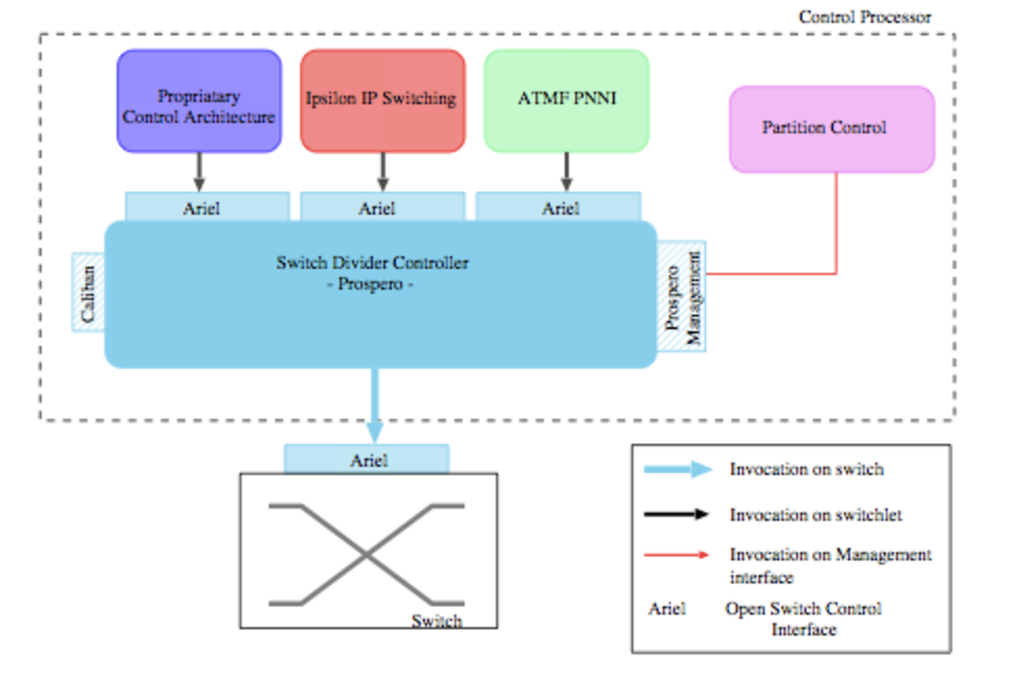
\includegraphics[width=0.7\textwidth]{Background/BackgroundFigs/tempest_arch}
\caption{Tempest switch architecture~\mycite{UCAM-CL-TR-450}}
\label{fig:background:tempest_arch}
\end{center}
\end{figure}

Active Networks focused extensively on Ethernet technologies and strived to
develop protocol evolvability. A similar approach was developer in the
University of Cambridge for the DCAN~\mycite{dcan} project, focusing though
primarily on control evolvability and network virtualisation in ATM networks.
DCAN tried primarily to simplify the control plane of ATM devices, in order to
support network multi-functionality. Similar efforts were developed by IETF
through the General Switch Management Protocol (GSMP)~\mycite{RFC3292}.

\mycite{Rooney1998} presented Tempest, a novel ATM switch architecture, which
enabled clean separation between the control and forwarding plane of an ATM
switch. Similar to the SDN approach,  the control plane was centralised in a
single programmable entity, which could implement intelligent and dynamic
forwarding.  The implementation of Tempest was logically divided between three
subsystems, depicted in Figure~\ref{fig:background:tempest_arch}. The figure
presents how a single switch is able to function in parallel as an IP router, an
ATM switch and a Hollowman controller~\mycite{Rooney1997}, a devolved ATM
control framework. 

\paragraph{Prospero Switch Divider} 

The \emph{Prospero} abstraction provides a mechanism to virtualise ATM switch
resources into multiple virtual switches, called \emph{switchlets}, through a
resource control interface.  A switchlet controls a subset of the switch ports,
VCI and VPI mappings, packet buffer and bandwidth. Prospero used the ATM QoS
principles to implement packet buffer and bandwidth virtualization.
Fundamentally, Prospero is responsible to map the control interface, exposed to
controllers, with the underlying switch functionality. 

\paragraph{Ariel Switch Independent Control Interface} 

Switchlets exposed forwarding control through the Ariel Interface. The Ariel
Interface organises network control through five control objects:
\emph{Configuration}, \emph{Port}, \emph{Context}, {\it Connections}
\emph{Statistics} and \emph{Alarms}.  The Configuration object provided details
for the switch configuration, the Port object provided primitive controllability
of ports (e.g.~state, loopback functionality), the Context object enabled QoS
policy control, the Connection object exposed control of VPI/VCI mappings, the
Statistics object exposed packet and byte counters and the Alarms object pushed
state change notifications to the controller. Tempest switches executed an Ariel
server and translated Ariel request to Prospero control requests. Ariel
fundamentally was an abstraction layer between the switch silicon and the
Prospero control interface. 

\paragraph{Caliban Switch Management Interface}

In addition to network control, Tempest also supported evolved network
management, through the Caliban interface. The interface functionality is
similar to the SNMP protocol. Caliban provides fine level SNMP-style
information, as well as, higher level aggregation operations over the switch
state. 

In addition to the redefinition of the network control abstraction, Tempest also
proposed a relaxed network resource management scheme.  Specifically, the
architecture proposed a measurement-based admission control mechanism for
circuit establishment~\mycite{Lewis1998}. The measurement scheme redefined the
static resource allocation scheme in ATM network, and used effective bandwidth
measurement techniques to estimate available resources and provide higher
utilisation of network resources, with minimum relaxation of the QoS guarantees. 

Tempest defined a highly efficient network control abstraction, which motivated
modern network control approaches, like the SDN, to reimplement it over Ethernet
devices.  The simplicity of the control abstraction, permitted
integration of the technology with existing forwarding devices  and enabled line
rate forwarding and efficient resource control.  Nonetheless, its strong
reliance on the ATM technology made the approach less relevant for the modern
Ethernet-dominated networks~\mycite{Crosby2002}. 

\subsection{SDN}\label{sec:background:sdn} 

SDN~\mycite{sdn}, the most recent network control paradigm, provides a pragmatic
approach to control evolvability. SDN employs  a clean separation between the
control and the forwarding plane of a network device. The control logic is
removed from the network device and implemented by a separate service.  A well
defined protocol establishes the integration between the two entities. 

The SDN paradigm is motivated by relevant earlier attempts in network
programmability(Active Networks and DCAN), but follows an evolutionary approach.
The paradigm is motivated by two key observations.  Firstly, the evolution of
computer networks has collapsed the layers of the OSI and TCP/IP model.
Production networks use network devices (e.g.~firewall, NAT, layer-5 switches)
which operate on multiple layers of the network and engage extensively in layer
violation.  The SDN paradigm provides a unifying cross-layer control model which
fits such functionality under a single interface.  Secondly, although network
complexity has increased, network devices still expose stand-alone,
decentralised and inflexible configuration mechanisms (e.g.~remote logic, CLI
interfaces), and employ proprietary control protocols, which reduce device
interoperability within the network. The SDN architecture establishes
centralised and unified management, supporting high control reactivity.  The \of
protocol is currently the pre-dominant implementation of the SDN paradigm.

\subsubsection*{\of protocol} 

\begin{figure}
  \begin{center}
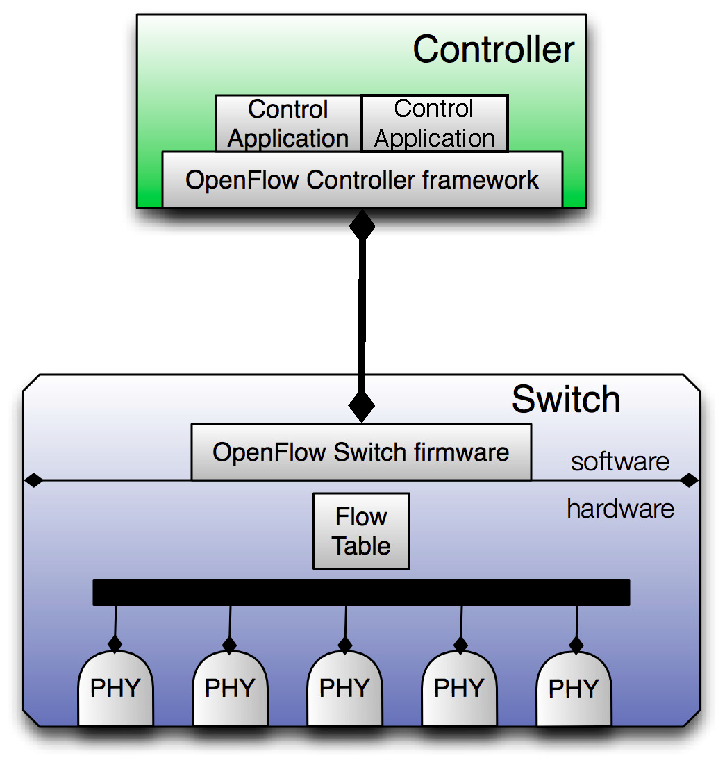
\includegraphics[width=0.5\textwidth]{Background/BackgroundFigs/openflow-schema}
\caption{A schematic representation of a basic \of setup}
\label{fig:background:openflow-schema}
\end{center}
\end{figure}
\begin{table}
  \begin{minipage} []{0.49\textwidth} 
    \begin{tabular}{|p{4cm}  | p{2cm} |} 
      \hline
      Field & OpenFlow Version \\ 
      \hline
      src \& dst MAC addr. & 1.0~\footnote{SInce version 1.1 the protocol
        permits masked mac address matching} \\ \hline
      input port & 1.0 \\ \hline
      VLAN ID & 1.0 \\ \hline 
      VLAN PCP & 1.0 \\ \hline
      MPLS label & 1.1 \\ \hline
      MPLS class & 1.1 \\ \hline 
      IPv4 src/dst addr. & 1.0 \\ \hline
      IPv4 proto & 1.0 \\ \hline
      ARP opcode & 1.0 \\ \hline 
      ARP src/dst IPv4 address & 1.0 \\ \hline 
      ARP src/dst MAC address & 1.2 \\ \hline 
    \end{tabular}
  \end{minipage}
  \begin{minipage} []{0.49\textwidth} 
    \begin{tabular}{|p{4cm}  | p{2cm} |} 
      \hline
      Field & OpenFlow Version \\  \hline
      IPv4 ToS & 1.0 \\ \hline 
      ICMPv4 Type \& Code & 1.0 \\ \hline
      TCP/UDP/SCTP src/dst port & 1.0 \\ \hline
      metadata & 1.1 \\ \hline
      IPv6 src/dst addr. & 1.2 \\ \hline
      IPv6 flow label & 1.2 \\ \hline
      ICMPv6 type \& code & 1.2 \\ \hline
      ICMPv6 Network Discovery target address & 1.2 \\ \hline
      ICMPv6 Network Discovery src/dst MAC address & 1.2 \\ \hline
    \end{tabular}
  \end{minipage}
    \caption{\of tuple fields} \label{tbl:background:openflow_tupple}
\end{table}
  \begin{table}
  \begin{minipage} [b]{0.49\textwidth} 
    \begin{tabular}{| p{4cm} | p{6cm}  | p{1.5cm} |} 
      \hline
      Field & operation & OpenFlow Version \\ \hline
      OUTPUT & output packet to a port & 1.0 \\ \hline
      SET\_QUEUE & output packet to a port queue & 1.0 \\ \hline
      SET\_VLAN\_VID & modify VLAN id & 1.0 \\ \hline 
      SET\_VLAN\_PCP & modify VLAN PCP & 1.0 \\ \hline
      SET\_DL\_SRC SET\_DL\_DST & modify src/dst mac addr. & 1.0 \\ \hline
      SET\_NW\_(SRC,DST) & modify IPv4 src/dst addr. & 1.0 \\ \hline
      SET\_NW\_TOS & modify IPv4 ToS & 1.0 \\ \hline
      SET\_NW\_ECN & modify IPv4 ECN bits & 1.1 \\ \hline
      SET\_TP\_(SRC,DST) & modify TCP/UDP/SCTP src/dst port & 1.0 \\ \hline
      COPY\_TTL\_(OUT,IN) & copy TTL value for IPv4 tunnels & 1.1  \\ \hline
      SET\_MPLS\_LABEL & modify MPLS label & 1.1 \\ \hline
      SET\_MPLS\_TC & modify MPLS traffic class & 1.1 \\ \hline
      (SET,DEC)\_MPLS\_TTL & modify/decrement MPLS TTL & 1.1 \\ \hline
      (PUSH,POP)\_VLAN & Add/remove a VLAN header & 1.1~\footnote{\of 1.0 defined
        a primitive to remove a VLAN header only} \\ \hline
      (PUSH,POP)\_MPLS & add/remove MPLS tag & 1.1 \\ \hline
      (SET,DEC)\_NW\_TTL & modify/decrement IPv4 TTL value & 1.1 \\ \hline
      (PUSH,POP)\_PBB & remove/add a PBB service tag & 1.3 \\ \hline

    \end{tabular}
  \end{minipage}
  \caption{\of available packet actions} \label{tbl:background:openflow_actions}
\end{table}

The \of protocol was originally defined by the \of Consortium, an organisation
of academic institutes, but currently the protocol development is steered by the
ONF, a standards definition committee comprised of academic institutions ,
service providers and network vendors. \of has been a highly successful approach
to network control. \of support is readily available in a series of production
devices, as well as, in large enterprise
networks~\mycite{google_of,Kobayashi:vn}.

Figure~\ref{fig:background:openflow-schema} presents an elementary \of topology,
consisting of two entities: the \textit{controller} and the \textit{switch}. The
two entities communicate over a TCP \textit{control channel}.  The \of controller
executes the network control logic and disseminates it to switches over
the control channel. The controller is usually divided in two layers. A controller
framework encapsulates the low level \of processing logic and exposes a higher
level abstraction to the developer.  Table~\ref{tbl:controller} presents a
complete list of available \of control frameworks.  The network control is
implemented in modules running over the controller framework. 


The \of switch, also called \textit{datapath}, abstracts the control of a
forwarding device. It consists of a set of \textit{flow tables}
and a set of \textit{ports}. The flow table is a memory module containing flow
entries which encode the active network policy. The data of a flow entry can be
decomposed in three structures: the flow tuple, the flow statistics and the flow
action list.  The tuple defines packet matches using header fields to group packets in
flows.  The fields of the tuple has evolved over the years and
Table~\ref{tbl:background:openflow_tupple} presents the match tuple fields
in each protocol version. Each tuple is associated with a field mask and permits
wildcard matching.  Flow statistics store packet and byte counters for each
flow. The action list, contains the list of actions applied to each matched
packet.  We present in Table~\ref{tbl:background:openflow_actions} the packet
processing actions defined by the \of protocol.  The protocol defines a simple
packet processing algorithm.  For each packet, the datapath extracts a set
of header fields and matches them against the entries of the flow tables.  If a
matching flow is found, then the flow statistics are updated and the action list
is applied on the packet. If there is no matching entry in the flow table, then
the packet is sent to the controller. The implementation of the \of switch
abstraction in production switches is usually split between the hardware and
software plane of the device. An \of agent runs on the switch co-processor,
translating \of operations in ASIC configuration.  

%% describe here how \of functionality is split between the switch. Maybe this
%% is irrelevant 
%% The control plane of the switch implements the translation of the \of protocol
%% into data path modifications.  It provides access and modification functionality
%% to the switch configuration and the flow table. The switch is able also to
%% propagate autonomously information and exceptions to the controller. 

The protocol defines a number of message types to control datapath resources.
\of messages can be grouped in two categories: \emph{Forwarding control} and
\emph{Switch configuration}. The rest of the section presents further details on
available \of messages and discusses the evolution of the protocol.  We focus
our protocol presentation on version 1.0 of the protocol.  ONF has releases
three revisions of the protocol, version 1.1, 1.2 and 1.3, which change
significantly the protocol specification. Nonetheless, the majority of
production systems support version 1.0.

\paragraph{Forwarding control}

\of supports two main control modes: \emph{reactive} and \emph{proactive}
control. In reactive control, the switch forwards every unmatched packet to the
controller, which is responsible to respond with appropriate modification in the
flow table. The protocol defines the {\tt pkt\_in} message to encapsulate the
header of a data plane packet when forwarded to the controller and the {\tt
  flow\_mod} message, to manipulate the flow table. The reactive control
approach provides fine control over the traffic dynamics, but introduces
significant load on the control plane. In proactive control, the controller is
responsible to pre-install all required flows in the flow table and avoid any
packet handling exceptions. The \of protocol provides the
\texttt{flow\_stats\_req/flow\_stats\_resp},
\texttt{port\_stats\_req/port\_stats\_resp} and
\texttt{aggr\_stats\_req/aggr\_stats\_resp} controller messages to poll for flow
and port statistics and infer network resource allocation. In order to ensure
operational atomicity, the protocol provides the
\texttt{barrier\_req/barrier\_reply} message to synchronise message execution
between the controller and the switch. A {\tt barrier\_reply} is send by a
switch as a response to a {\tt barrier\_req} from the controller, when all
previous operations are processed.  Finally, the \of protocol provides two
additional message types to enhance control capabilities: the {\tt pkt\_out} and
the {\tt flow\_removed}. The {\tt pkt\_out} message enables the controller to
inject traffic in the data plane and the {\tt flow\_removed} message can notify
the controller when a flow entry is removed from the flow table.

\paragraph{Switch configuration} 

Apart from the control of the flow table, the \of protocol provides switch
configuration capabilities. A controller can use the {\tt
  switch\_config\_req/switch\_config\_resp} message types, to discover the
switch operational support of \of functionality.  In addition, the protocol
provides capabilities to control port state with the {\tt port\_mod} message
type. The switch is also able to notify the controller when a port changes its
state (e.g.~link is detected to be inactive in the physical layer) with the {\tt
  port\_status} message. In the recent revisions of the protocol, the steering
committee has introduced the capability to control per port traffic shaping
queues. 

\paragraph{Protocol evolution} 

Since the specification of the version 1.0 of the protocol, the \of steering
committee has produced 3 non-backward compatible protocol revisions. This
protocol evolution is driven both by the osmosis between the hardware and
software community and the introduction of new deployment use-cases. 

Version 1.1  modifies the main protocol processing pipeline and exposes a switch
abstraction which matches better the design of an ASIC\@. Specifically, the packet
lookup process searches sequentially, instead of parallel, between the switch
flow tables.  The packet must match an entry in each of the tables otherwise a
{\tt pkt\_in} message is generated. In addition, in order to persist partial
results between tables, the protocol define a 64-bit per-packet metadata field
and the action list is augmented with operations over the metadata field and
over the table search process (e.g.~terminate lookup, skip table).  Secondly,
the protocol introduces a primitive to express multipath support in the protocol
using a new forwarding table, the group table.  Group table entries consists of
group entries containing flow actions and an assigned output port. A flow table
entry can forward a matching packet to a group entry. The group selection action
can forward a packet to all the buckets of the entry (ALL) or to a random
bucket, similar to Equal Cost Multiple Path routing (ECMP)~\mycite{RFC2992}
functionality, (SELECT) or select a specific bucket (INDIRECT) or to the first
group entry with a non-blocked output port (FAST\_FAILOVER).  Thirdly, the
protocol introduces MPLS support.

Version 1.2 of the protocol extends data plane protocol support. This revision
introduces support for IPv6 and Provider Bridge Network (PBB - Mac-in-Mac)
traffic. In addition the protocol uses a flexible Type-length-format (TLV) for
flow tuple definitions.  Finally, the protocol defines a model for efficient
multi-controller switch connectivity, in an effort to improve control channel 
resilience.

Version 1.3 introduces protocol support of QoS control. The protocol defines a
new table abstraction, the metering table, which contains queue definitions. In
addition, this protocol defines a control plane improvement using multiple
parallel control channels to the controller, in order to parallelize {\tt
  pkt\_in} transmission, and defines a mechanism to support message
fragmentation.  

Because the protocol complexity has increased significantly in the recent
versions of the protocol, the vision for future \of functionality, is to
differentiate support between devices and optimize only a subset of the
functionality. For example, a firewall device can support only network and
transport layer field match to improve flow table capacity. 

\section{SDN applications} \label{sec:background:ofapp}

\begin{table}
  \center
  \begin{tabular}{|c  | l |}
    \hline
    Language & controller \\
    \hline
    Python & NOX~\mycite{nox}, POX~\mycite{pox}, Pyretic~\mycite{Monsanto13} \\
    C++ & NOX~\mycite{nox} \\
    JAVA & Maestro~\mycite{cai2011}, Floodlight~\mycite{floodlight} \\
    Haskell & Nettle~\mycite{nettle} \\
    C & Mul~\mycite{mul} \\
    Javascript & Nodeflow~\mycite{nodeflow} \\
    Ruby & Trema~\mycite{trema} \\
    \hline

  \end{tabular}
  \caption{List of \of controller organised by programming language}
  \label{tbl:openflow-controller}
\end{table}
 
\begin{table}
  \center
  \begin{tabular}{|c  | c | c |}
    \hline
    Vendor & Model & \of version \\
    \hline

    HP & 8200zl, 6600, 6200zl, 5400zl, and 3500/3500yl & v1.0 \\
    Brocade & NetIron CES 2000 Series & v1.0 \\
    IBM & RackSwitch G8264 & v1.0 \\
    NEC & PF5240, PF5820 & v1.0 \\
    Pronto & 3290, 3780 & v1.0 \\
    Juniper & Junos MX-Series & v1.0 \\
    Pica8 &  P-3290, P-3295, P-3780 and P-3920 & v1.2 \\
    \hline
  \end{tabular}
  \caption{List of hardware switches with \of support }
  \label{tbl:openflow-switch}
\end{table}
 
The SDN paradigm has proven extremely effective both for the network community
and the industry. A number of vendors provide production-level hardware SDN
support (Table~\ref{tbl:openflow-switch}), while the SDN community provides \of
support for the majority of programming languages
(Table~\ref{tbl:openflow-controller}).  In this section we iterate a series of
network problem classes and present the design of a series of effective SDN
applications which address these problems.

\subsection{Network Virtualisation Applications}

The introduction of OS virtualization and the subsequent rise of the cloud
computing paradigm has created new opportunities for ICT to reduce
infrastructure costs and provide high level of resilience to applications.
Although OS virtualisation platforms, like Xen, provide high precision resource
allocation and performance isolation, there is still a significant mismatch in
the network abstraction.  The introduction of the SDN abstraction in the
datacenter provides novel opportunities to extend the virtualisation abstraction
in network resources. 

\mycite{flowvisor-ccr} presented \flv, an early network virtualisation approach
based on \of.  \flv functions as an \of proxy between switches and controllers
and manages to transform control over a set of switches into a single big
virtual switch abstraction.  \flv employs a simple network topology discovery
and resource control mechanism, while appropriate message processing allows to
translate the view between the two abstractions.  The administrator can
partition the \of tuple, delegate network control to different controllers and,
effectively, allow multiple tenants to exercise network control for their own
network subnet over the same network infrastructure.  FlowVisor quickly
transformed into a network product by BigSwitch. Furthermore,
\mycite{Corin12}~develop a topology virtualisation extension for \flv.
FlowN~\mycite{Drutskoy13} follows a different approach and integrate
virtualisation in the  programming framework.  The framework uses VLAN tags to
multiplex data plane traffic and synchronizes controller state through an SQL
database. Finally, Nicira provides the Nicira Network Virtualization Platform
(NVP), a production level network virtualisation and control isolation
framework, which though is proprietary and implementation details are
undisclosed. 

\subsection{Security and Access Control Applications}

% Network security is currently a primary requirement for network functionality.
SDN provides fast  prototyping for secure network applications and
unprecedented control reactivity to threat detection framework.
Ethane~\mycite{casado07:_ethan}, an  early attempt to define the SDN
abstraction, established a policy expression language to control interactions
between user identities and network services.  \mycite{Ballard10} focus on the
problem of effective network monitoring and present OpenSAFE, a policy
expression language for efficient traffic interception and inspection.  Finally,
\mycite{Porras12} present FortNOX, an security extension  for network
virtualisation applications. FortNOX enables users to assign priorities and
roles to control applications and resolves automatically policy inconsistencies. 
 
\subsection{Load Balancing Applications}

The high popularity of network services with global scope has introduced a
requirement for novel indirection mechanisms, with high responsiveness and
resilience. Current approaches employ proprietary load balancing devices, which
distribute dynamically user request between servers.  SDN can integrate the
indirection functionality in the network fabric. \mycite{Wang11}~present an
in-network proactive load balancing framework which uses the range of the \of
wildcard matching to distribute client load between servers.
\mycite{Handigol09,Handigol10} follow a reactive approach to the problem. For
each new client, their Plug-and-Serve controller chooses on-the-fly a
destination server, based on an allocation algorithm and the overall system
load.

\subsection{Inter-domain and Intra-domain Routing}

The SDN community has developed a series of applications to improve the performance
of existing control plane protocols.  \mycite{Rothenberg12} present an integration
of the Quagga~\mycite{quagga} routing framework with the \of protocol, in an
effort to revisit Route Reflectors in BGP routing~\mycite{RFC4456}. Similarly,
\mycite{Kotronis12} revisits the problem of BGP routing instabilities and propose a
framework for \of-based BGP calculation offloading to third parties.

The SDN has also motivated explorations on forwarding state compressibility.
\mycite{Sarrar12} present a library which exposes an \of-based FIB abstraction
for routing applications.  The library at run-time analyses the FIB table and
the traffic pattern and calculates the minimum set of flow entries which can
server a specific subset of the traffic on the fast-path of the network.
\mycite{Yu10} present DIFANE, a valiant routing framework achieving significant
FIB table compressibility.  The proposed mechanism uses the \of abstraction to
partition effectively the network IP space and aggregate subsets of the FIB on
each network device. 

\subsection{Network Management Applications}

SDN control primitives can support the development of innovative network
management frameworks. One the first efforts was the Onix management
framework~\mycite{Koponen10}. Onix provides a centralised control abstraction
through its development API, which at run time was transparently distributed
across the network. 

The SDN paradigm has found significant applications in the formalisation of the
network management. \mycite{Foster11} present Frenetic, a declarative
programming language for network control policy providing inherent support for
significant network control programming requirements, like race conditions.
\mycite{Monsanto12a} developed NetCore, a policy expression language providing
dynamic policy adaptation to traffic and topology changes and automatic
optimization of the forwarding state. \mycite{Guha13} introduced verfiability to
the NetCore language, while \mycite{Monsanto13} proposed an extension which
provide seamless integration between control applications. Such control
abstraction have also been discuss in the context of network upgradability.
\mycite{Reitblatt12} present a verifiable framework which ensured network
operability during updates. Finally, \mycite{Voellmy12} present a declarative
policy language exposing a functional reactive programming model and providing
development flexible. 

\subsection{Energy Control Applications}

In the recent years, energy consumption has become an important measure of
efficiency for a system architecture. Currently the network is estimated to
contribute approximately 20\% of the total power consumption of a data-center.
Unlike CPUs which can reduce power consumption when idle, network cards exhibit
a constant high power consumption, due to continuous physical layer frame
synchronisation. As a result the most efficient mechanism to reduce network
power consumption is to shutdown interfaces.  \mycite{Heller10} present a
power-aware control plane architecture, build on top of the \of abstraction. The
application takes advantage of link redundancy and turns off interfaces when
network utilisation is low. 

\subsection{Network Debugging and Measurement Applications}

The SDN paradigm, as well as, the \of abstraction provide novel mechanisms for
network troubleshoot and debug. \mycite{Wundsam11} present OFRewind, a mechanism
to intercept and record network policy inconsistencies for debugging purposes.
\mycite{Handigol12b}~present ndb, a control plane debugger which replicate the
gdb abstraction for \of applications. Ndb enables developers to register data
plane breakpoint conditions and receive rich state information when these
conditions are met.  Finally, a number of applications have been proposed to
enable control plane monitoring in order to detect potential networks
misconfigurations.  \mycite{Khurshid12} present an \of proxy service which
detect flow modifications which create forwarding policy inconsistencies.
\mycite{Canini12} present a model checking mechanism which uses symbolic
execution to detect flow modifications which create significant inconsistencies
in the data plane forwarding.  Recent efforts in remote network debugging have
introduced \of-based solutions for home networks.  \mycite{Calvert10} propose a
network controller providing precise home network logging, in an effort to
enable ISPs to troubleshoot connectivity problems. 

% \mycite{opentm-pam}, 
%   OFRewind, ndb, end, VeriFlow~\mycite{Khurshid12}
% Home instrumenting~\mycite{Calvert10}, An \of-based instrumentation
%         router for home networks. ISP can receive accurate network information 
%         from the home network and troubleshoot easier home problems.

\subsection{Resource Control Applications}

SDN reactivity enables fine level resource control and a number of applications
have been developed for datacenter environments.  \mycite{Al-Fares10} presented
Hedera, a novel datacenter control architecture providing better network
utilisation in comparison to the ECMP~\mycite{RFC2992} network load balancing
mechanism. Hedera uses the \of flow statistics to discover progressively
network-limited flows and reroute them over underutilised network paths.
\mycite{Benson11} presented a network load distribution mechanism designed to
exhibit fairness towards short-lived flows. \mycite{Even12} employ \of in a
network embedding mechanism for datacenter job assignments and provide strong
resource guarantees.

Resource control has also been proposed in the context of home networks.
\mycite{Yiakoumis11} propose home network virtualisation in an effort to improve
resource allocation on the edges and enable core infrastructure sharing between
ISPs.  Furthermore, \mycite{Yiakoumis12} evolve this idea and introduce a simple
user interface which can translate user resource requirement into ISP wide
network policies. 

\subsection{Mobility Applications}

The SDN paradigm provides novel control capabilities in mobile networks.
\mycite{Huang10} present PhoneNet, a mobile application development framework
which provides the ability for dynamic multicast groups setup.
\mycite{Yap09,Yap10} present OpenRoads, a network control plane for wireless
network, enabling seamless Access Point~(AP) hand-overs and network
virtualisation.  Finally, \mycite{Li12} discuss SDN applicability for
cellular networks.

\subsection{Network Simulation}

Currently a number of large-scale shared experimentation infrastructures provide
\of support. The GENI testbed~\mycite{geni} funded by the NSF and the Ofelia
testbed~\mycite{ofelia} funded by the EU FP7 framework provide network and
computing resource to run large-scale experiments for free.  \mycite{Erickson11}
present Virtue, a large-scale Xen-based emulation framework which uses the \of
protocol to enable scalable user experimentation with network topologies and VM
placements in a multi-tenant data center environment. Similarly,
Mininet~\mycite{Lantz10,Handigol12}  provides a scalable platform  for \of
experimentation and reproducibility. Mininet uses the LXC~\mycite{lxc} Linux
user-space virtualisation framework and network namespaces to run large scale
topologies in a single host and experiment with network functionality.  Mininet
has been used in Stanford Computer Science department to introduce of students
to recent research efforts~\mycite{cs244}. 

\section{Conclusions}

In this section we provided an in-depth analysis of available network control
mechanisms.  We motivated the discussion by presenting a generic architectural
model for network devices and highlighted the inherent limitations for network
control. Furthermore, we presented the current production  control mechanisms
and, motivated by their limitations, we presented three experimental network
control frameworks, namely Active Networks, Devolved Control for ATM Network and
Software Defined Networking. Finally, we provided an extensive presentation of
recent efforts to improve modern network functionality through control plane
redesign. In the next chapter we present an extensive study on the scalability
of the SDN paradigm. 
